\section{Introduction}

%motivation
The physical laws of motion say that an accelerating car consumes more fuel than a car driving at a constant velocity. %TODO: Citation
If one wants to safe fuel, one should therefore try to accelerate as little as possible. 
However, several factors in todays traffic hinders drivers in driving at a constant velocity. 
These are for example interlacing roads, blocking cars, traffic incidents and of cause traffic lights. 
It is esimated at 1.8 bilion danish kroner is lost on fuel each year on vehicles stopping for red light in traffic lights in Denmark \cite{Vejdir}.

%the problem of traffic lights
Traffic lights hinders the flow of traffic as it stops cars arriving from one direction in order to allow other cars to drive through the intersection.
Each direction of the intersection is given a time period in which cars are allowed to pass through the intersection. 
From a drivers perspective it is only posible to guess when the light is going to change based on what he has seen so far. 
This is often difficult, and will in many case mean that the driver will have to make full stop at the traffic light. This is bad for the fuel economy.
Modern traffic lights have sensors known as \textit{induction loops} that can detect cars driving on the roads.
These sensors are used to regulate the signals in relation to the number of cars approaching the intersection \cite{Vejdir}.
If it is possible to reduce the stop-and-go behaviour at traffic lights, it might be possible to reduce the fuel consumption.
%section describing terms of traffic traffic light phase, cycle time ect


%model discribing what we do


%problem of not knowing how many other cars are wating in line
The system proposed in this article is designed on the basis that not every vehicle will be using it. 
Because of this, we cannot rely on communication between vehicles and therefore we do not know how many cars are going to be waiting in line for a green light. %TODO this depents on access to induction loop data
Hence we cannot predict the precise distance to the position at a traffic light were the driver must stop before due to blocking cars.

\begin{figure}[htb]
\centering
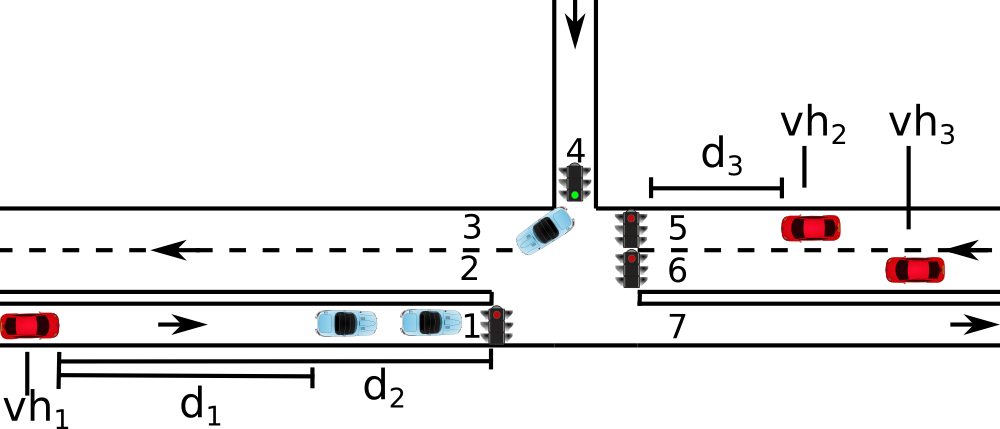
\includegraphics[width=0.5\textwidth]{images/introNetwork.png}
\caption{Eksample network}
\label{fig:Introduction:network}
\end{figure}

\begin{table}[h]
\centering
\begin{tabular}{|l|l|}
\hline
from & to \\ \hline
1 & 7 \\ \hline
4 & 3 \\ \hline
4 & 7 \\ \hline
5 & 3 \\ \hline
6 & 2 \\ \hline
\end{tabular}
\caption{Connection table of the network shown in Figure \ref{fig:Introduction:network} }
\label{tab:Introduction:connectionTable}
\end{table}


%section describing problem with sensors
A traffic light using only a timer to regulate the trafic is relativly easy to predict if the phases and cycle time is known. 
However, when we introduce induction loops that are are effected by vehicles ariving in an unpredicteble pattern, then the traffic light will also to some extent become unpredicteble. 

%describe why we do simulation 
The focus of this article is to investigate whether it is possible to reduce fuel consumption at traffic ligths by mathcing the speed to the traffic lights. We investigate this through simulations, but will reald world map data, traffic data and traffic light programs, %TODO check we do this
both with crossing traffic and road-side senors.
%To investigate the extent of this problem we create simulations based on real world map data, traffic data and traffic light programs. 
We use the traffic simulator SUMO (Simulation of Urban Mobility)\cite{sumo} interfaced via TraCI (Traffic Control Interface)\cite{traci} which is a full scall microscopic traffic simulator.

%TODO: outline of the article
//Outline of the article





